
\documentclass[xcolor=dvipsnames]{beamer}

\usepackage{latexsym}
\usepackage{braket}
\usepackage{graphicx}
\usepackage{amsfonts}
\usepackage{amsmath}
\usepackage{verbatim}
\usepackage{amssymb}
\usepackage{amsthm}
\usepackage[english]{babel}
\usepackage[utf8]{inputenc}
\usepackage{listings}
\usepackage{color}
\usepackage{float}
\usepackage{geometry}
\usepackage{algorithm}
\usepackage{algpseudocode}
\usepackage{pdfpages}
\usetheme{default}
\usecolortheme[named=Brown]{structure} 
\setbeamertemplate{frametitle}[default][] 
\definecolor{lightbrown}{rgb}{0.933,0.890,0.773}

\setbeamerfont{section in head/foot}{size={\fontsize{8}{8}}}
\setbeamercolor{section in head/foot}{bg=lightbrown!5}
\setbeamercolor{head/foot}{ bg=Brown!45}
\setbeamercolor{frametitle}{fg=Brown, bg=lightbrown!30}
\setbeamercolor{block title}{bg=lightbrown}
\setbeamercolor{block body}{bg = lightbrown}
\setbeamertemplate{blocks}[rounded][shadow=true]


\setbeamertemplate{headline}{%
\leavevmode%
  \hbox{%
    \begin{beamercolorbox}[wd=\paperwidth,ht=3.5ex,dp=1.125ex, plus1fil]{palette quaternary}%
    \insertsectionnavigationhorizontal{\paperwidth}{}{\hskip 0cm}
    \end{beamercolorbox}%
  }
}

\makeatletter
    \newenvironment{withoutheadline}{
        \setbeamertemplate{headline}[default]
        \def\beamer@entrycode{\vspace*{-\headheight}}
    }{}
\makeatother


\logo{
\includegraphics[height=0.8cm]{unipi}\hspace{0.1cm}
\includegraphics[height=0.8cm]{anna}}
\setbeamertemplate{navigation symbols}{}


\title[framework]{
\includegraphics[height=1.3cm]{unipiinit2}
\includegraphics[width=0.5cm]{space}
\includegraphics[height=1.3cm]{annainit}\newline \newline
A Framework for static allocation of parallel OpenMP code on multi-core platforms\\}
\author[]{Giacomo Dabisias, Filippo Brizzi}
\institute[unipi]{
  Universit\`a degli studi di Pisa,\\
  Scuola Superiore Sant'Anna\\
  Pisa,Italy\\[1ex]

}


\definecolor{blue}{RGB}{0,0,180}
\definecolor{darkblue}{RGB}{72,61,139} 
\definecolor{green}{rgb}{0,0.4,0}
\definecolor{gray}{rgb}{0.5,0.5,0.5}
\definecolor{darkgray}{rgb}{0.4,0.4,0.4}
\definecolor{mauve}{rgb}{0.58,0,0.82}
\definecolor{black}{rgb}{0,0,0}
\definecolor{purple}{RGB}{138,43,226}
\definecolor{ocra}{RGB}{218,165,32}
\definecolor{maroon}{rgb}{0.5,0,0}
\definecolor{darkgreen}{rgb}{0,0.5,0}
\definecolor{indianred}{RGB}{178,34,34}


\lstdefinelanguage{CCC}{ 
  breakatwhitespace=false,         
  breaklines=true,                 
  captionpos=b,                   
  frame=single,                    
  keepspaces=true,                 
  numbers=left,                    
  numbersep=5pt,                   
  numberstyle=\tiny\color{gray}, 
  rulecolor=\color{black},         
  showtabs=false,                  
  stepnumber=1,                    
  tabsize=2,                       
  title=\lstname,                   
  basicstyle=\scriptsize,
  stringstyle=\color{ocra},
  morestring=[b]",
  identifierstyle=\color{black},
  morecomment=[l][\color{maroon}]{pragma\ },
  morecomment=[l][\color{gray}]{//},
  morecomment=[s][\color{gray}]{/*}{*/},
  keywordstyle=[1]\color{blue},
  keywords=[1]{int,float,char, class, void, unsigned, struct, bool},
  keywordstyle=[0]\color{indianred},
  keywords=[0]{include,for,if,while,return,public,break}
}

\lstdefinelanguage{AST}{ 
  breakatwhitespace=false,         
  breaklines=true,                 
  captionpos=b,                   
  frame=single,                   
  keepspaces=true,                 
  rulecolor=\color{black},         
  showtabs=false,                  
  tabsize=2,                       
  title=\lstname,                   
  morekeywords={A}, 
  keywordstyle=\color{blue},
  language=C++,
  morecomment=[s][\color{gray}]{<}{>},
  stringstyle=\color{ocra},
 basicstyle=\color{black}\footnotesize\tiny
}



\date[February 2014]{February 28, 2014}

\begin{document}

\begin{withoutheadline}
\begin{frame}
  \titlepage
\end{frame}
\end{withoutheadline}

\begin{section}{Introduction}





\begin{frame}{\hskip 0.3cm Context and motivations}

Real-time systems are moving towards multicore architectures. The majority of multithread/core libraries target high performance systems. 

\begin{itemize}

\item Real-time applications need strict timing guarantees and predictability.

 \begin{center} Vs \end{center}

\item High performance systems try to achive a lower computation time in a best efford manner.

\end{itemize}

There is no actual automatic tool which has the advantages of HPC with timing contrains.

\end{frame}









\begin{frame}{\hskip 0.3cm Objectives and Design Choice: OpenMP and Clang}


OpenMP 

\begin{itemize}

\item Minimal code overhead.

\item Well spread standard.

\item Opensource and supported by several vendors like Intel and IBM.

\end{itemize}

Clang

\begin{itemize}

\item Provides code analysis and source to source translation capabilities.

\item Modularity and great efficency.

\item Opensource and supported by several vendors like Google and Apple.

\end{itemize}

\end{frame}









\begin{frame}{\hskip 0.3cm OpenMP }

Multiple threads of execution perform tasks defined by directives.

\begin{itemize}
\item Each directive applies to  a block of C++ code embedded in a scope.

\item Allows nested parallelism though nested directives.

\item Clauses allow variables management.
\end{itemize}

\begin{block}

$\#$pragma omp directive-name [clause[ [,] clause]...] new-line

\end{block}

Choosen subset for the framwork:

\begin{itemize}

\item Control directives : parallel, sections, single.

\item Working directives : task, section, for.

\end{itemize}

\end{frame}










\begin{frame}{\hskip 0.3cm OpenMP}

\begin{figure}
\centering
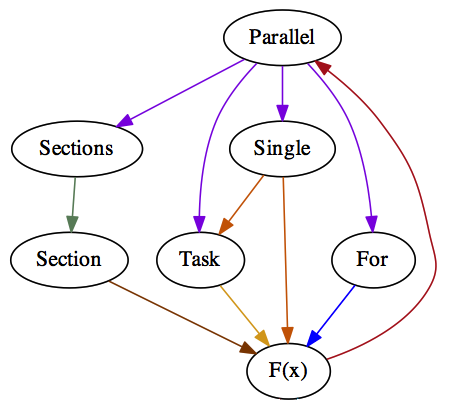
\includegraphics[scale = 0.45]{ompstructure}

\end{figure}

\end{frame}














\begin{frame}{\hskip 0.3cm Clang}

Clang and OpenMP:
\begin{itemize}
\item In July 2013 Intel released a patched version of Clang which fully supports the OpenMP 3.3 standard. 
\end{itemize}

The strength of Clang lies in its implementation of the Abstract Syntax Tree (AST).
\begin{itemize}

\item Closely resembles both the written C++ code and the C++ standard.

\item Clang’s AST nodes are modeled on a class hierarchy that does not have a common ancestor.

\item Hundreds of classes for a total of more than one hundred thousand lines of code.

\end{itemize}
\end{frame}










\begin{frame}{\hskip 0.3cm Clang - AST}

To traverse the AST, Clang provides the RecursiveASTVisitor class.
\begin{itemize}

\item Very powerful and easy to learn interface

\item Possibility to create a custom visitor that triggers only on specific nodes.


\end{itemize}

Clang supports the insertion of custom code through the Rewriter class.
\begin{itemize}

\item Allows insertion, deletion and replacement of code.

\item Operations are performed during the AST visit.

\item A new source file with all the modifications is generated at the end of the visit.

\end{itemize}

\end{frame}











\begin{frame}[fragile]{\hskip 0.3cm Clang - AST}

\begin{columns}

\begin{column}{4cm}
\begin{lstlisting}[language=CCC]
class A {
public:
  int x;
  void set_x(int val) {
       x = val * 2;
  }	
  int get_x() {
      return x;
  }
};
int main() {
    A a;
    int  val = 5;
    a.set_x(val);
}
\end{lstlisting}
\end{column}

\begin{column}{7.3cm}

\begin{lstlisting}[language=AST]
TranslationUnitDecl
|-CXXRecordDecl <clang_ast_test.cpp:2:1, line:13:1> class A
| |-CXXRecordDecl <line:2:1, col:7> class A
| |-AccessSpecDecl <line:3:1, col:7> public
| |-FieldDecl <line:4:2, col:6> x 'int'
| |-CXXMethodDecl <line:5:2, line:7:2> set_x 'void (int)'
| | |-ParmVarDecl <line:5:13, col:17> val 'int'
| | `-CompoundStmt <col:22, line:7:2>
| |   `-BinaryOperator <line:6:3, col:13> 'int' lvalue '='
| |     |-MemberExpr <col:3> 'int' lvalue ->x
| |     | `-CXXThisExpr <col:3> 'class A *' this
| |     `-BinaryOperator <col:7, col:13> 'int' '*'
| |       |-ImplicitCastExpr <col:7> 'int' <LValueToRValue>
| |       | `-DeclRefExpr <col:7> 'int' lvalue ParmVar 'val' 'int'
| |       `-IntegerLiteral <col:13> 'int' 2
...
\end{lstlisting}
\end{column}

\end{columns}


\end{frame}








\end{section}
\begin{section}{Framework}











\begin{frame}{\hskip 0.3cm The framework}
\end{frame}












\begin{frame}{\hskip 0.3cm General Design}
\end{frame}












\begin{frame}{\hskip 0.3cm Big-graph image}
\end{frame}












\begin{frame}{\hskip 0.3cm Simple example}
\end{frame}












\begin{frame}{\hskip 0.3cm Pragma extraction}
\end{frame}












\begin{frame}{\hskip 0.3cm Intrumentation for profiling}
\end{frame}












\begin{frame}{\hskip 0.3cm Intrumentation for profiling - Annotated example}
\end{frame}












\begin{frame}{\hskip 0.3cm Flow graph}
\end{frame}












\begin{frame}{\hskip 0.3cm Scheduler}
\end{frame}












\begin{frame}{\hskip 0.3cm Scheduler - Search tree}
\end{frame}












\begin{frame}{\hskip 0.3cm Scheduler - Constraints check}
\end{frame}












\begin{frame}{\hskip 0.3cm Scheduler - (Cetto \& Chetto)}
\end{frame}












\begin{frame}{\hskip 0.3cm Final execution}
\end{frame}












\begin{frame}{\hskip 0.3cm Final execution - Intrumentation}
\end{frame}












\begin{frame}{\hskip 0.3cm Final execution - Run-time}
\end{frame}












\begin{frame}{\hskip 0.3cm Fianl execution - (thread pool)}
\end{frame}












\begin{frame}{\hskip 0.3cm Final execution - (multiple job queues)}
\end{frame}












\begin{frame}{\hskip 0.3cm Final execution - (synchronization)}
\end{frame}












\end{section}
\begin{section}{Test}












\begin{frame}{\hskip 0.3cm General structure}
\end{frame}












\begin{frame}{\hskip 0.3cm General structure -(graph of the test code)}
\end{frame}












\begin{frame}{\hskip 0.3cm Results}
\end{frame}












\begin{frame}{\hskip 0.3cm Results - (some tables and graphs)}
\end{frame}












\begin{frame}{\hskip 0.3cm Results - (total completion time)}
\end{frame}












\begin{frame}{\hskip 0.3cm Results - (service time - boxplot)}
\end{frame}












\begin{frame}{\hskip 0.3cm Results - (Jitter)}
\end{frame}












\begin{frame}{\hskip 0.3cm Results - Comments}
\end{frame}












\end{section}
\begin{section}{Conclusion}












\begin{frame}{\hskip 0.3cm }
\end{frame}












\end{section}

\end{document}
